% --------------------------------------------
%		CAPITOLO 4 
%---------------------------------------------
\chapter{VTX detector} \label{ch:VTX}


This chapter describes the vertex detector upgrade of Belle II, VTX. We will go through the VTX concept and layout, designed with a different geometry with respect VXD and with a new pixel sensors (OBELIX). We will discuss the motivations for some of the design choices and present some of the detector performance studies demonstrating the robustness against backgrounds.


%---------------------------------------------
%			4.1
%---------------------------------------------
\section{VTX Layout and mechanical structure}

As previously discussed (\autoref{ch:upgrade}), reaching full luminosity will entail higher backgrounds and will probably require a re-design of the interaction region. It is therefore necessary to use a radiation-hard technology, with high granularity to reduce occupancy, and with a reduced material budget to improve the already excellent performance of VXD.


\begin{figure}[h!]
\centering
\subfigure[Concept of VTX layout with 5 barrel layers, filling \newline the current VXD volume.]{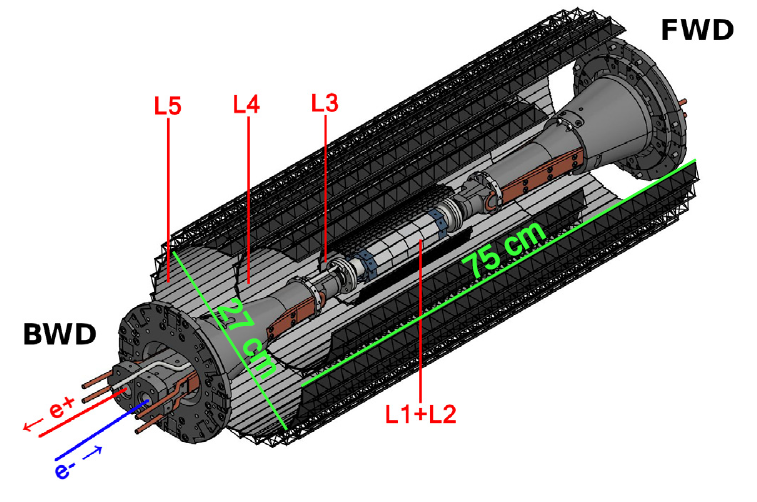
\includegraphics[scale=.65]{VTX_layers}}
\subfigure[End view of the VTX detector for layer 3 at \SI{39}{mm} from the IP.]{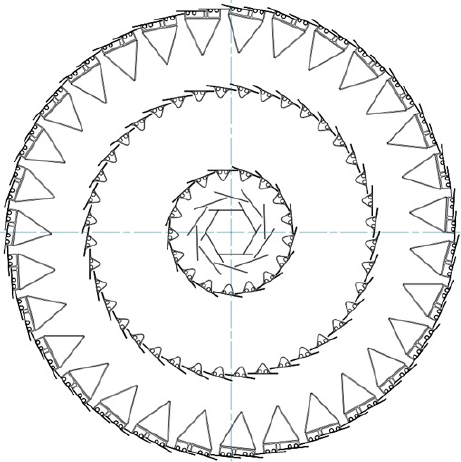
\includegraphics[scale=.65]{VTX_layers_endview}}
\caption{VTX detector layout.}
\label{fig:VTX_layers}
\end{figure}


The VTX project aims to replace the VXD with a fully pixelated detector based on Depleted Monolithic Active Pixel Sensors (DMAPS) arranged in five layers at different distance from the beam pipe (\autoref{fig:VTX_layers}) \cite{BelleIIVTX:2023szr, F.Forti:3930}. The radii and the number of the layers are currently subject to several  studies and simulations, in order to achieve an optimized arrangement (shown in~\autoref{tab:layers_tab}). 
%There are two options for the third layer (3a and 3b), as reported in~\autoref{tab:layers_tab}
Currently two layers are planned in the innermost part (\textit{i}VTX) and three in the outer part (\textit{o}VTX). The active length of the ladders varies from 12 to \SI{70}{cm} to cover the required acceptance of \ang{17}~<~$\theta$~<~\ang{150}.\\
It is important to try to reduce the material budget, in order to minimize the multiple Coulomb scattering which particularly affects the very soft particles produced in Belle II, down to \SI{50}{MeV}. By using the MAPS sensors, it is expected a reduction of the overall material budget down to less than 2\% of radiation length, against the present 3\% of VXD.

\begin{table}[h!]
\centering
\begin{tabular}{C{3cm}|C{0.8cm}|C{0.8cm}|C{0.8cm}|C{0.8cm}|C{1.2cm}||C{1.2cm}|C{0.8cm}||C{1.2cm}}
\hline
\hline
Layer & 1 & 2 & 3a & 4 & 5 & Total & 3b & Total \\
\hline
\hline
Radius (mm) & 14.1 & 22.1 & 39.1 & 89.5 & 140.0 & & 69.1 & \\
\hline
\# Ladders & 6 & 10 & 17 & 40 & 31 & 104 & 30 & 117 \\
\hline
\# Sensors/ladder & 4 & 4 & 7 & 16 & \numproduct{2 x 24} & 2311 & 12 & 2552 \\
\hline
Mat. Budget ($X_{0}$) & 0.1 & 0.1 & 0.3 & 0.5 & 0.8 & 1.8 & 0.4 & 1.9 \\
\hline
\hline
\end{tabular}
\caption{The VTX detector main parameters with the two options (3a and 3b) for the radius of the middle layer. From~\cite{F.Forti:3930}.}
\label{tab:layers_tab}
\end{table}


\subsection{iVTX}

The \textbf{\textit{internal}VTX} consists of the first two detector layers assembled with a self-supported air-cooled all-silicon ladder concept, where four contiguous sensors are diced out of a single wafer, thinned and interconnected with post-processed redistribution layers. They are designed to be at 14 and \SI{22}{mm} respectively from the beam pipe, and target an individual material budget of about 0.1\% radiation length. 
This is achievable because the overall surface of these layers is moderate, below \SI{400}{cm^{2}}, the sensor power dissipation is expected to be low, and the connections needed for the operation to be only a few. Air cooling should be a workable solution to remove the heat produced.


\begin{figure}[h!]
\centering
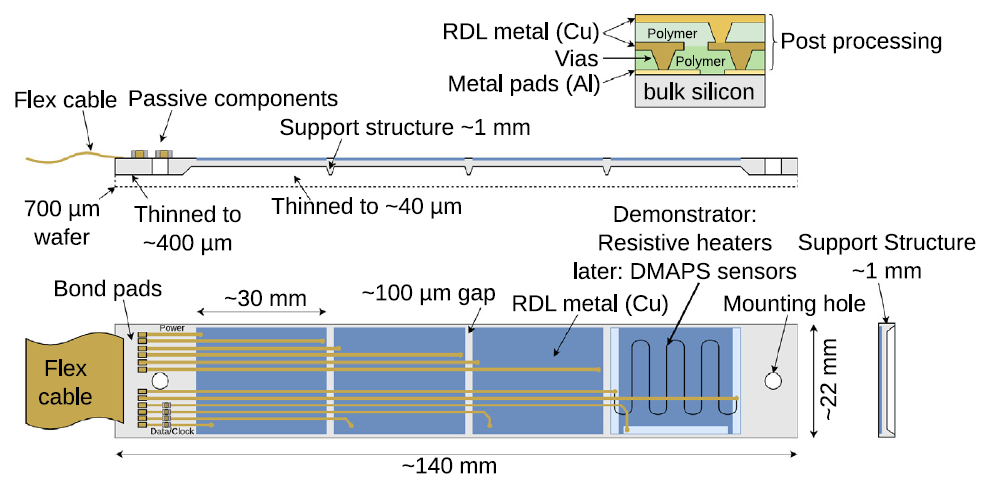
\includegraphics[scale=.65]{iVTX}
\caption{Sketch of the all-silicon ladder concept of the iVTX. Four dummy sensors are shown in blue on the silicon support in grey. The yellowish lines instead, indicate power and data transmission lines. Power is delivered to the ladder by a flex cable, which also transmits data to and from the chips in the final one.}
\label{fig:iVTX}
\end{figure}

The ladder has to be equipped with four OBELIX chips and thinned to \SI{50}{\micro m} except in some border regions, where a few hundreds of \unit{\micro m} are necessary to ensure mechanical stability. 
In order to interconnect the sensors along the ladder and provide a unique connector at the backward end, during the post-processing metal strips are etched on the redistribution layer (RDL). The latter has the main purpose to route power and data via impedence-controlled transmission lines to a flex cable, added at the end of the ladder.
After the RDL processing, the ladder is thinned as discussed above. Mounting holes will be added via laser-cutting.


\autoref{fig:iVTX} shows a sketch of the iVTX demonstrator ladder (currently under production), \SI{140}{mm} long and \SI{22}{mm} wide (grey). Instead of the actual sensors, it is equipped with four dummy chips with a length of about \SI{30}{mm} (blue), holding resistors to mimic the expected heat load to test the air cooling system and more generally to characterized the electrical, mechanical and thermal performance of the ladder.
A redistribution layer for power and data is also added to the demonstrator, to connect the chips with a flex cable at the end of the ladder (yellowish lines). The wafer thickness is reduced to \SI{400}{\micro m}, while the sensitive areas are thinned down to \SI{40}{\micro m} with the purpose to test the mechanical integrity of the whole structure.

The R\&D is ongoing and the full-silicon ladder concept is currently being assessed with industrial partners. The first thin ladders have been produced and characterised with different thicknesses and geometries.

Several tests are focused on evaluating power delivery efficiency, the quality of the signals which travel through the ladder and also the process used to fully assembly it. 
\autoref{fig:iVTX_eye} shows eye diagrams from simulation with a transfer rate of \SI{640}{Mbps}, indicating that \SI{320}{Mbps} of data rate will be possible.

\begin{figure}[h!]
\centering
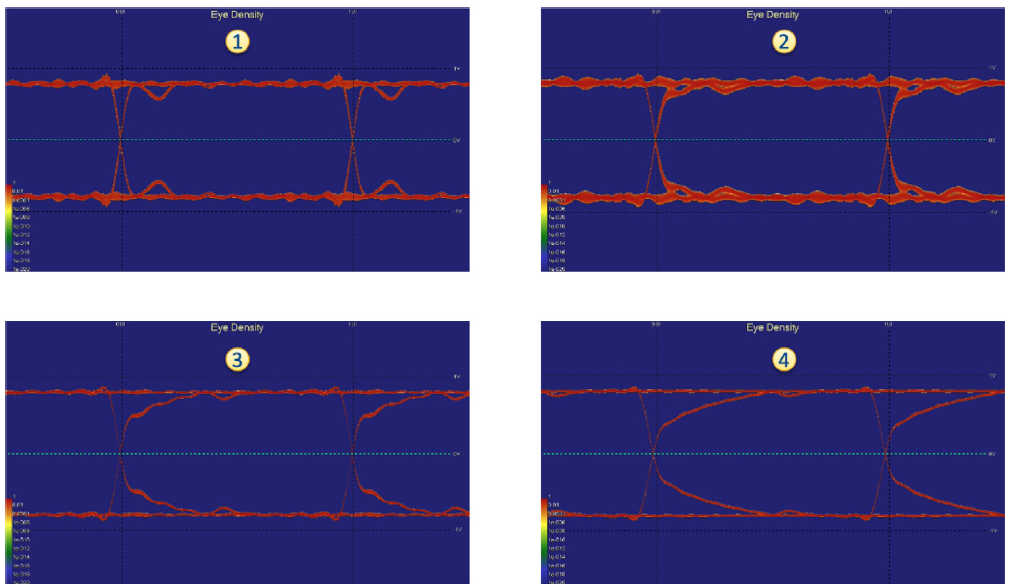
\includegraphics[scale=.7]{iVTX_eye}
\caption{Eye diagrams of the iVTX data transmission lines at four different locations on the ladder. They represent the overlap of multiple samples of the output of transmission line triggered by the clock cycle. From~\cite{BelleIIVTX:2023szr}.}
\label{fig:iVTX_eye}
\end{figure}

Moreover, it has been demonstrated that air at the temperature of \SI{15}{\degreeCelsius} and flowing with a speed of \SI{10}{m/s} succeeds to cool a single inner module, assuming power is uniformly dissipated on the sensor surface. The maximum temperature reached is \SI{20}{\degreeCelsius}. 

Through very first estimates it is expected that an equivalent section of 6 tubes with \SI{10}{mm} of diameter is necessary to expel the heat from the inner layers, roughly equal to \SI{65}{W}. So it is essential to design a mechanical structure which provides for the space needed to the tubes in order to bring the air at the IP and also compatible with the new interaction region.


\subsection{oVTX} \label{sec:oVTX}

The \textbf{\textit{outer}VTX} consists of three layers respectively at radii of 39 or 69, 89 and \SI{140}{mm} from the interaction point. Because of the larger distance required to cover the acceptance, they cannot be self-supporting. They follow a more traditional approach, inspired by the design developed for the ALICE ITS2 \cite{Fantoni:2020iyr}. Each ladder is water cooled and supported by a light carbon fiber support structure, which provides the mechanical stiffness. Its truss design is shown in~\autoref{fig:oVTX} : \SI{70}{cm} long and \SI{5.8}{g} of weight, it is able to support more than 40 sensors in two rows next to each other with a small overlap, leading to a material budget of 0.3\% $X_{0}$ for the first layer, 0.5\% $X_{0}$ for the second and 0.8\% $X_{0}$  for the outermost one.

\begin{figure}[h!]
\centering
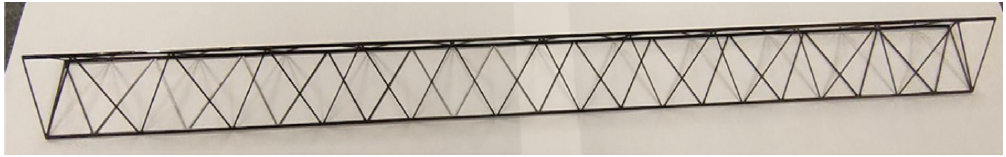
\includegraphics[scale=.7]{oVTX}
\caption{Prototype of the layer 5, called \textit{truss}, which is the longest, made from thin carbon fibre structures.}
\label{fig:oVTX}
\end{figure}


For the cooling of the ladder a cold-plate concept is under development (\autoref{fig:oVTX_coldplate}), on which the sensors are glued and that in turn is installed on the \textit{truss}. For each row there is a polymide cooling tube that runs over all the sensors and turns back at the other end, so that the cooling circuit connections are on the same side. Two flexible printed circuits are wire-bonded to the OBELIX chips and provide the connection to the readout.


\begin{figure}[h!]
\centering
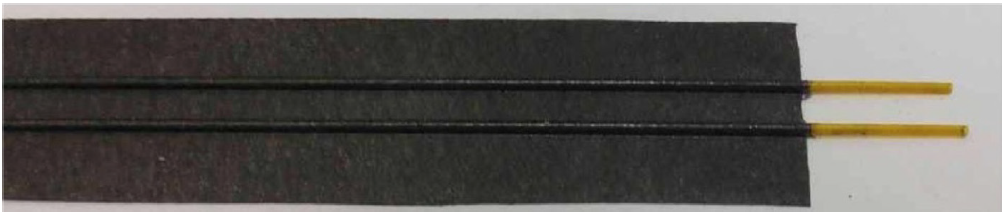
\includegraphics[scale=.7]{coldplate}
\caption{A prototype of the cold-plate for cooling. One coolant tube(golden) is connected to the cold plate(black) and turns \ang{180} on the other end (not shown) so that the coolant flows in both directions and thus leaves on the same side it starts.}
\label{fig:oVTX_coldplate}
\end{figure}

For layer 3 instead, only one flex printed circuit cable in the backward side is considered, to leave more space forward for other possible services and accelerator components. For the third layer two different solutions are under study: at radius of \SI{39}{mm} e \SI{69}{mm} respectively. 
In~\autoref{fig:ladders} schematic examples of some design hypotheses are displayed. 

\begin{figure}[h!]
\centering
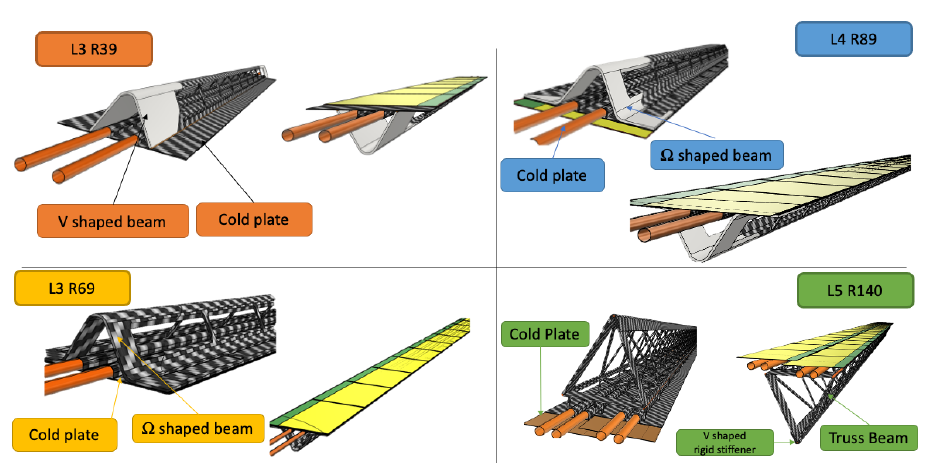
\includegraphics[scale=.8]{ladders}
\caption{Schematic view of possibile solutions for the three outermost layers.}
\label{fig:ladders}
\end{figure}


\autoref{fig:oVTX_5} shows the several substructures described before, that constitute a ladder of the outermost layer 5. From bottom to top the carbon fibre structure, two cold-plates for the two neighbouring sensor rows (indicated as "Chips", in grey) and the flex cables for power and data transmission (green) follow one another. 


\begin{figure}[h!]
\centering
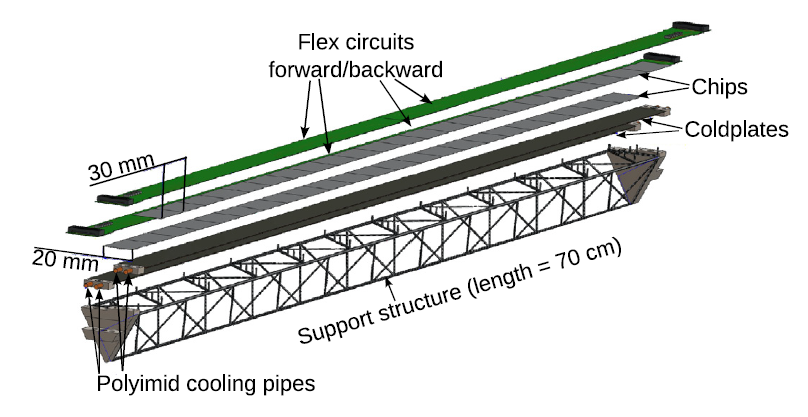
\includegraphics[scale=.8]{oVTX_5}
\caption{An exploding drawing of a fully assembled layer 5 ladder.}
\label{fig:oVTX_5}
\end{figure}


The carbon fiber support structure and the flex cables have been designed and fabricated for layer 5, which is also the longest. Services for the last two layers, like electrical connections and cooling, can be provided both on forward and backward sides.
A Multiline Power Bus has been realized to power each OBELIX chip along the ladder. \\

Mechanical tests have been performed showing that the first resonance frequency is at \SI{200}{Hz}, which is safely far from the frequencies of the typical earthquakes in Japan.
To reduce as much as possible the material budget, the transmission lines and the flex cables must be as thin as possible, but they also have to ensure safe data transmission.

In~\autoref{fig:oVTX_eye} the resulting eye diagram from testing the signal integrity of one of the \SI{35}{cm} long transmission lines for data transmission rate of \SI{500}{Mbps} is shown. This result demonstrates that the bandwidth is large enough to allow the needed \SI{160}{Mbps} for data transmission.


\begin{figure}[h!]
\centering
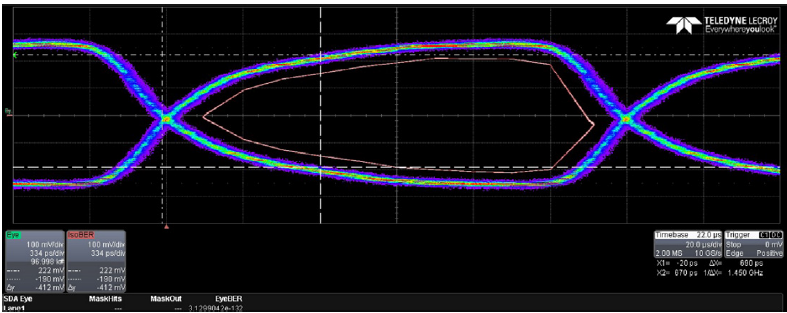
\includegraphics[scale=.8]{oVTX_eye}
\caption{Eye diagram for the oVTX transmission line signal integrity of the layer 5 flex cable. From~\cite{BelleIIVTX:2023szr}.}
\label{fig:oVTX_eye}
\end{figure}


In addition, thermal tests have been performed for the last layer prototypes using kapton heaters to emulate the power dissipation of the chips. The coolant (demineralized water) has been set to a temperature of \SI{10}{\degreeCelsius} at the beginning, the environment at \SI{20}{\degreeCelsius} with a negative pressure of \SI{0.2}{bar}. Results have demonstrated that for three different configurations of the flow (such as monodirectional, bi-directional and with an U-turn at one end) the average temperature remains below \SI{24}{\degreeCelsius} with a maximum gradient of $\Delta T \approx$ \SI{4}{\degreeCelsius} along the full length of the ladder. 

All these investigations validate the design of the longest ladder, which is the most challenging, and therefore the possibility to operate the chips safely.


%---------------------------------------------
%			4.2
%---------------------------------------------
\section{Performance simulation}


As we have seen in~\autoref{ch:upgrade}, increasing the luminosity implies higher level of machine related background and larger doses of radiation, especially in the inner layers of the detector. 
For these reasons simulations and studies are focusing on ensuring that the main physics goals of the experiment will be achieved despite the more severe working conditions. 

The VTX detector, with high granularity in both space and time and thin sensors, could bring significant improvements in tracking efficiency and resolution especially at low momentum, in the impact parameter resolution, and in the robustness against backgrounds. Moreover, better vertexing performance entails not only improved time-dependent analyses of B and D mesons, but also an enhanced capability to distinguish among different decay topologies, and a more powerful rejection of background events.


\subsection{VTX geometries}

Two different VTX geometries are currently under study, which differ only in the position of the third layer (\autoref{fig:ladders}).  

The \textit{\textbf{nominal}} geometry is expected to maximize the track impact parameter resolution and it places the third layer at \SI{39}{mm} from the IP.
The \textit{\textbf{alternative}} geometry instead, aims to improve the $K_{S}^{0}$ reconstruction efficiency and the third layer is located at \SI{69}{mm} from the IP.

Simulations are ongoing to compare the performance of these two different layouts with that of the current Belle II detector (utilizing a full Geant4 simulation of the detector in the study of specific decay modes of interest)~\cite{Belle-II:2023lba}. Moreover, the different machine background predictions are also simulated, to compare the detector performance under different background conditions. 

\subsection{Tracking efficiency at low momentum and impact parameter resolution}

Tracking efficiency at low momentum is one of the areas where the VTX upgrade provides the most promising results, particularly for the \textit{soft pions} originated from the decays of $D^{*\pm}$ mesons.

Studies are based on the reconstruction of the decay chain $B^{0}~\rightarrow~D^{*-}l^{+}\nu$, with $D^{*-}~\rightarrow\bar{D}^{0} \pi^{-}_{soft}$ and $\bar{D}^{0}~\rightarrow~K^{+} \pi^{-}$ or $K^{+} \pi^{-} \pi^{+} \pi^{-}$. All background scenarios mentioned in~\autoref{sec:bkg_predictions} are considered in the evaluation of the \textit{nominal} VTX performance and they are compared with the nominal Belle II geometry in the intermediate (\textbf{v2}) background hypothesis.


\begin{table}[htbp]
  \begin{center}
    \begin{tabular}{l|c|c|c|c}
      \hline\hline
      & Belle II (v2) & VTX (v1) & VTX (v2) & VTX (v3) \\
      \hline\hline
      Generated events & 32533 & 32559 & 32559 & 30255 \\
      \hline
      Correctly reconstructed signal & 10059 & 16913 & 16848 & 15583 \\
      \hline
      Combinatorial & 28495 & 51375 & 51826 & 47527 \\
      \hline\hline
      Efficiency & 30.9\% & 51.9\% & 51.7\% & 51.5\% \\
      \hline
      Purity & 26.1\% & 24.8\% & 24.5\% & 24.7\% \\
      \hline\hline
    \end{tabular}
  \end{center}
   \caption{Reconstruction efficiency and purity for the the decay chain $B^{0} \rightarrow D^{*-}l^{+}\nu$, with $D^{*-} \rightarrow \bar{D}^{0} \pi^{-}_{soft}$ and $\bar{D}^{0} \rightarrow K^{+} \pi^{-}$, for the nominal Belle II detector at the intermediate background conditions (\textbf{v2}) and the nominal configuration of VTX in all three background scenarios.}
\label{tab:simulation_low_mom}
\end{table}


In~\autoref{tab:simulation_low_mom} the VTX reconstruction efficiency\footnote{Efficiency is defined as the ration between the number of correctly reconstructed signal events and the total number of candidates.}  in all three background hypotheses is reported, and it is improved by almost a factor 1.7 with respect to the nominal Belle II, with comparable purity\footnote{In a few words, the probability that a correctly reconstructed signal  is a ''signal event''.} . Moreover, efficiency remains practically stable in all background conditions, even in the most severe one.

This enhancement in tracking efficiency relies in particular on improved tracking efficiency for the $\pi_{soft}^{-}$ mesons, as we can see in~\autoref{fig:simulation_soft_pi} where the efficiency is shown as a function of momentum and polar angle.


\begin{figure}[h!]
\centering
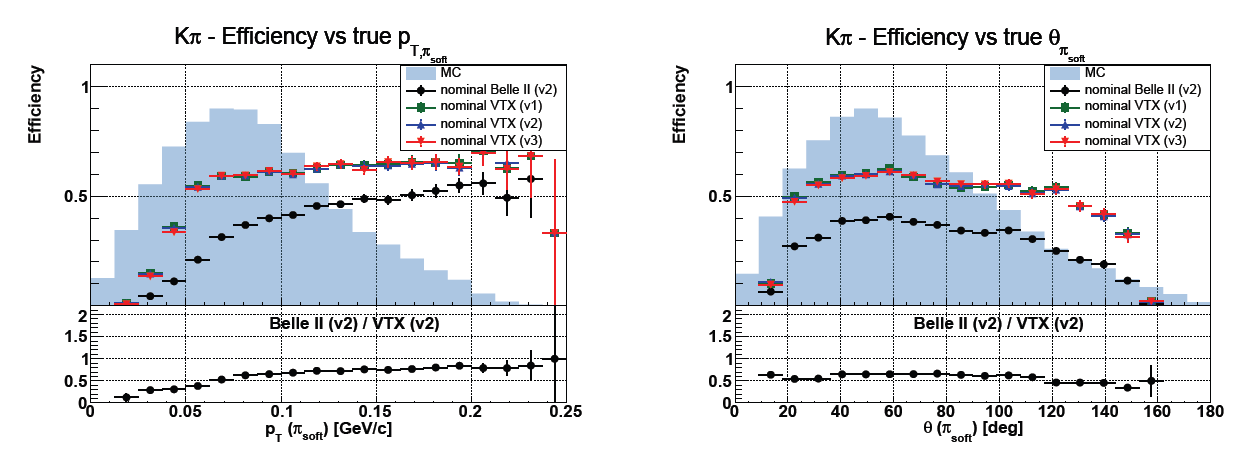
\includegraphics[scale=.65]{simulation_soft_pi}
\caption{Reconstruction efficiency of $B^{0} \rightarrow D^{*-}l^{+}\nu$ as a function of the transverse momentum of the $\pi_{soft}^{-}$ (from  $D^{*-} \rightarrow \bar{D}^{0} \pi^{-}_{soft}$) in the plot on the left and of the polar angle of the $\pi_{soft}^{-}$ on the right. 
The shaded blue histograms represents the momentum spectrum of the  $\pi_{soft}^{-}$.
The nominal Belle II geometry efficiency in the intermediate background scenario (\textbf{v2}) is represented by black dots and it is compared with the nominal VTX configuration in the optimistic (\textbf{v1}, green squares), medium (\textbf{v2}, blue upward pointing triangles) and pessimistic (\textbf{v3}, red downward
pointing triangles) background hypotheses. The bottom plots show the ration between nominal Belle II and nominal VTX in the \textbf{v2} background scenario. From \cite{F.Forti:3930}.}
\label{fig:simulation_soft_pi}
\end{figure}


\subsection{Vertexing resolution}

Studies on vertexing performance have been conducted using samples of one million $B^{0} \rightarrow J/\psi K_{S}^{0}$ events generated and reconstructed with all the aforementioned combinations.
The distributions of the decay vertex resolution $\sigma_{z}$ (i.e. the width of the distribution obtained considering the differences between the measured and the true simulated positions) along the \textit{z} axis of the B decay signal are shown in~\autoref{fig:simulation_vertex} .

\begin{figure}[h!]
\centering
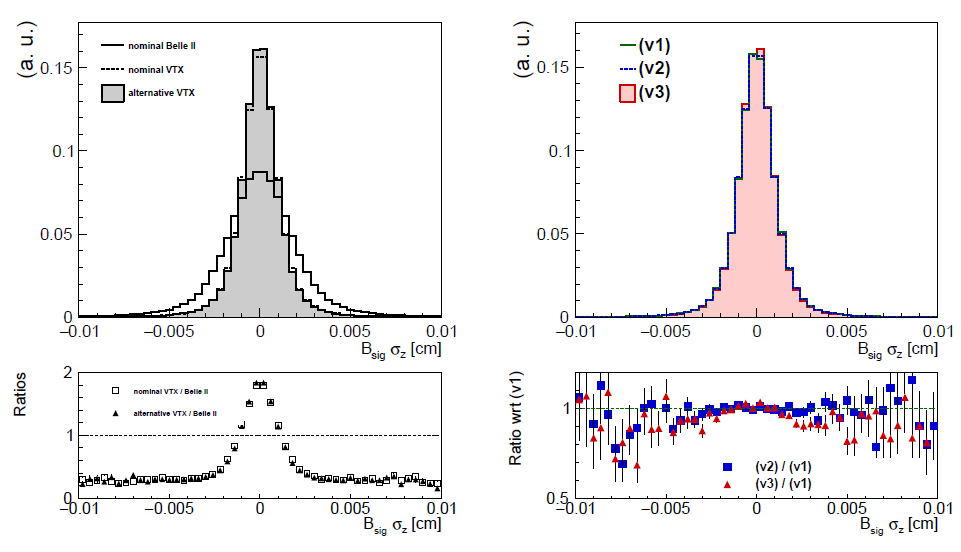
\includegraphics[scale=.75]{simulation_vertex}
\caption{On the left: comparison of the B decay vertex resolution along the \textit{z} axis in $B^{0} \rightarrow J/\psi K_{S}^{0}$ events for the nominal Belle II (solid line), nominal VTX (dotted line) and alternative VTX geometry (filled grey histogram). The bottom plot shows the ratio between the VTX geometries (empty squares the nominal one and filled triangles the alternative) and nominal Belle II. \\
On the right:  B decay vertex resolution along the \textit{z} axis for the nominal VTX geometry in the three background scenarios: optimistic \textbf{v1} (green solid line), intermediate \textbf{v2} (blue dotted line) and pessimistic \textbf{v3} (red filled histogram). The bottom plot represents the ratio between the two higher background scenarios and the optimistic one. From \cite{F.Forti:3930}.}
\label{fig:simulation_vertex}
\end{figure}

In~\autoref{tab:simulation_vertex_table} a summary of the results that shows that the new geometries achieve a better resolution on the B decay vertex of about 35\% on average and they also do not suffer of any significant degradation as the background conditions varies, unlike the nominal Belle II configuration.

\begin{table}[htbp]
  \begin{center}
    \begin{tabular}{l|c|c|c}
      \hline\hline
      $B_{sig}$ $z$ vertex resolution ($\mu$m) & Bkg (v1) & Bkg (v2) & Bkg (v3) \\
      \hline\hline
      Belle II & 21.9 & 23.0 & 24.9 \\
      \hline
      Nominal VTX & 14.5 & 14.4 & 14.1 \\
      \hline
      Alternative VTX & 14.4 & 14.3 & 14.0 \\
      \hline\hline
    \end{tabular}
  \end{center}
\caption{$B_{sig}$ vertex resolution along the \textit{z} axis for the three detector layouts and the three background scenarios.}
\label{tab:simulation_vertex_table}
\end{table}


Similar studies for the $K_{S}^{0}$ decay vertex resolution are displayed in~\autoref{fig:simulation_vertex_K} and in the same way, the upgraded geometries reach a better vertexing resolution with respect to the nominal Belle II detector, without any significant degradation as the backgrounds increase.

\begin{figure}[h!]
\centering
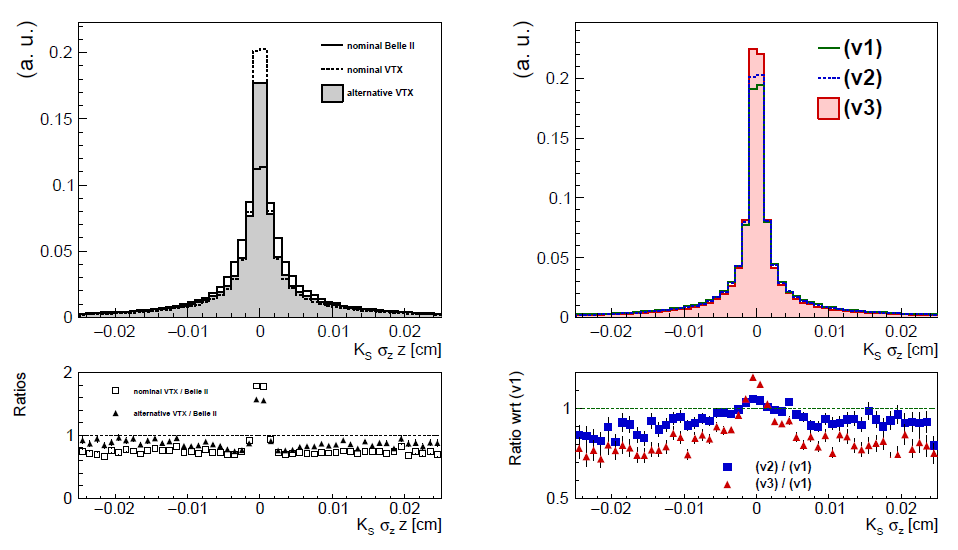
\includegraphics[scale=.75]{simulation_vertex_K}
\caption{On the left: comparison of the $K_{S}^{0}$ decay vertex resolution along the \textit{z} axis in $B^{0} \rightarrow J/\psi K_{S}^{0}$ events for the nominal Belle II (solid line), nominal VTX (dotted line) and alternative VTX (filled grey histogram). The bottom plot shows the ratio between the VTX geometries (empty squares for the nominal and filled triangles for the alternative) and nominal Belle II detector. 
On the right: $K_{S}^{0}$ decay vertex resolution along the \textit{z} axis for the nominal VTX in the three background scenarios: optimistic \textbf{v1} (green solid line), intermediate \textbf{v2} (blue dotted line) and pessimistic \textbf{v3} (red filled histogram). The bottom plot represents the ratio between the two higher background scenarios and the optimistic one. From \cite{F.Forti:3930}.}
\label{fig:simulation_vertex_K}
\end{figure}

\clearpage

%---------------------------------------------
%			4.3
%---------------------------------------------
\section{OBELIX chip design}

The VTX detector is designed with a single type sensor optimized for the specific needs of Belle II, called OBELIX (Optimized BELle II pIXel sensor) and currently under development, based on fast and high granular Depleted Monolithic Active Pixel Sensors (DMAPS). The sensor design comes from an evolution of TJ-Monopix2 chip, whose characterization will be discussed in~\autoref{ch:TJ2}. Both of them are fabricated in a modified TowerJazz Semiconductor \SI{180}{nm} CMOS process.


\subsection{Sensor specification}

The main design specifications for the OBELIX chip are listed in~\autoref{tab:obelix_features}.


%\begin{comment}
\begin{table}[h!]
\centering
\begin{tabular}{c|c}
\hline 
\hline
Pixel pitch & 30 to \SI{40}{\micro m} \\
\hline
Matrix size & 512 rows\numproduct{_x 928} to 752 columns \\
\hline
Time stamping & 25 to \SI{100}{ns} precision over 7 bits\\
\hline
Signal Time over threshold & 7 bits\\
\hline
Output bandwidth & 320 to \SI{640}{Mbps}\\
\hline
Power dissipation & 100 to \SI{200}{mW/cm^{2}}\\
\hline
Radiation tolerance & \SI{1}{MGy} and \SI{e14}{n_{eq}/cm^{2}}\\
\hline
\hline
\end{tabular}
\caption{Designed specifications of the OBELIX sensor.}
\label{tab:obelix_features}
\end{table}
%\end{comment}

\begin{comment}
\begin{table}[h!]
\centering
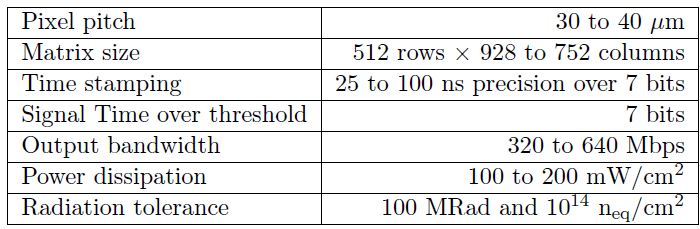
\includegraphics[scale=.7]{obelix_features}
\caption{Designed specifications of the OBELIX sensor.}
\label{tab:obelix_features}
\end{table}
\end{comment}

The pixel pitches\footnote{The distance between the centers of two contiguous pixels.} are designed to be from \SI{30}{\micro m} to \SI{40}{\micro m} in both directions. This range is necessary to achieve a spatial resolution below \SI{15}{\micro m}, which is required to obtain sufficient tracking performance \cite{F.Forti:3930}.


Moreover the sensor thickness has to be below \SI{100}{\micro m} to respect the material budget constraint of 0.2\% $X_{0}$ (\SI{100}{\micro m} Si correspond to 0.1\% $X_{0}$) which is possible with the DMAPS technology. 
To deal with the target hit rate of \SI{120}{MHz/cm^{2}}, the timestamp clock signal can reach down to \SI{25}{ns}, even if studies have demonstrated that a window of \SI{100}{ns} (\textit{integration time}) is enough to limit to \SI{320}{Mbps} the data throughput at the same expected hit rate. The expected radiation tolerance must comply with the radiation robustness requirements mentioned in~\autoref{sec:VTX_requirements}.
All characteristics inspected above allow to realize a sensor with high granularity in both space and time.\\

With respect to TJ-Monopix2, which is equipped with a triggerless column-drain readout without memory at the periphery (\autoref{sec:TJ_arch}), OBELIX must have a triggered readout architecture to satisfy the needs of Belle II. The latency is fixed to \SI{10}{\micro s} and it might operate up to 30 KHz trigger rate.


Single Event Upset~\footnote{A Single Event Upset (SEU), also known as a Single Event Error (SEE), occurs if the charge released by ionizing particle, happens to be deposited close to a sensitive node of the device (RAM cell, register), causing a bit value to flip leading to corrupt information.} is a concern for future detector operation, therefore an important feature of the chip must be to ensure that the control system is able to reset the sensor registers to default operational values at least every minutes. The reset frequency will be chosen after the measurement of the SEU cross section with OBELIX and the comparison to the occurrence distribution of large energy loss in the experiment.
%but its size has not yet been quantified.

The power consumption is expected to be about \SI{200}{mW/cm^{2}}, a value which should allow air-cooling for the small areas corresponding to the two inner layers and liquid coolant for the outer ones. This relatively high value is necessary to obtain the required speed of the chip.


\subsection{Sensor implementation}

A schematic layout of the chip is shown in~\autoref{fig:obelix_scheme} . The sensor size is expected to be \numproduct{3 x 1.9}~\unit{cm^{2}}, with an active area of \numproduct{3 x 1.6}~\unit{cm^{2}} and an additional part in the periphery of about \numproduct{3 x 0.3}~\unit{cm^{2}}, dedicated to data pre-processing and triggering.

\begin{figure}[h!]
\centering
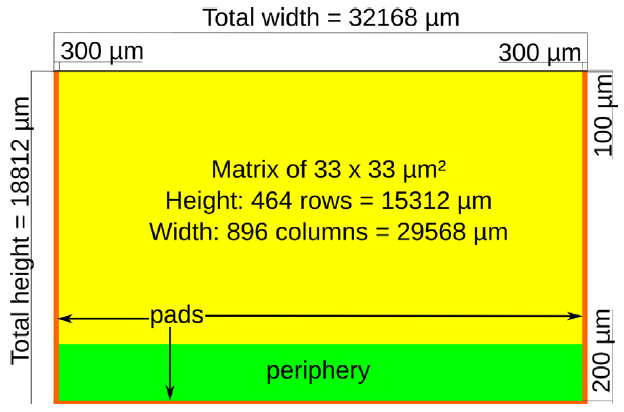
\includegraphics[scale=.7]{obelix_schematic}
\caption{OBELIX chip layout.}
\label{fig:obelix_scheme}
\end{figure}

As mentioned above, this new sensor is the development of TJ-Monopix2, whose characteristics fit already many of the Belle II requirements (\autoref{tab:obelix_specification}).\\


%\begin{sidewaystable}
\begin{table}
\centering
\begin{tabular}{lc|c}
\hline
\hline
 & Specification & TJ-Monopix2\\
\hline
Pixel pitch & $< 40 \mu m$ & $< 33 \mu m$ \\
Sensitive layer thickness & $< 50 \mu m$ & $30 \mu m$ and $ 100\mu m$ \\
Sensor thickness & $< 100\mu m$ & - \\
\hline
Hit rate capability in the matrix & $> 600$~MHz~cm$^{-2}$ & $> 600$~MHz~cm$^{-2}$ \\
\shortstack{Hit rate capability at the \\sensor output} & $>120$~MHz~cm$^{-2}$ & $\gg 100$~MHz~cm$^{-2}$ \\
Trigger delay & $>10 \mu s$ & - \\
Trigger rate & $30$~kHz & - \\
%(optional) Track-trigger capability & \rem{to fill} & - \\
Overall integration time & $<100$~ns & - \\
(optional) Time precision & $<50$~ns & - \\
\hline
Total ionizing dose tolerance & 100~kGy/year & 1~MGy/year \\
NIEL fluence tolerance & \SI{5 e 13}{n_{eq}/cm^2/year}  & \SI{1.5 e 15}{n_{eq}/cm^2/year} \\
SEU tolerance & flash configuration(~min$^{-1}$) & - \\
\hline
Matrix dimensions & around $30 \times 16 mm^{2}$ & $19 \times 19 mm^{2}$ \\
Overall sensor dimensions & around $30 \times 19 mm^{2}$ & $20 \times 19 mm^{2}$\\
Powering & through voltage regulators & - \\
Outputs & one at $<200 \rm{ MHz}$ & one at $160$~MHz \\
\hline
\hline
\end{tabular}
\caption{OBELIX sensor specifications, compared to the relevant specifications of the TJ-Monopix2 sensor.}
\label{tab:obelix_specification}
\end{table}
%\end{sidewaystable}



From TJ-Monopix2 design, the pixel size of \numproduct{33 x 33}~\unit{\micro m^{2}} is maintained, as well as the layout of both digital and analog parts (\autoref{sec:TJ}). Also the Time-Over-Threshold method to digitize the signal is preserved, with a bus width of 7 bit, together with the column-drain readout architecture implemented for pairs of columns. Other features which will be explained in depth in~\autoref{ch:TJ2}, have been maintained in the new design, like the 3-bit register dedicated to the threshold tuning, but with a larger range of correction (for the last bit). 
To aim at the integration time of \SI{100}{ns}, the clock frequency which defines the precision of TOT and BCID (that is the timestamp), has been decreased from 40 to \SI{20}{MHz}. Thus the current baseline for OBELIX timestamp precision is \SI{50}{ns}.

Additionally, two new modules have been added to the implementation, related to the Belle II trigger: the Trigger Logic Unit (TRU) and the Track Trigger Transmitter (TTT). 

\begin{description}
\item \textbf{Trigger Logic Unit (TRU)}
\end{description}

The TRU has the task to select the fired pixel information from the matrix which are in-time with the triggers sent by the Belle II system. For this purpose it employs two stages of memory (\autoref{fig:obelix_tru}): the first stage has to store the pixel information during the trigger delay; the second memory has to compare the BCID (Bunch Crossing ID) of the fired pixel with each trigger time information buffered in a dedicated global memory. When they have a match, the pixel data is transferred to the Transmission Unit (TXU). Considering the BCID time precision, the time integration of the OBELIX sensor becomes \SI{100}{ns}.

\begin{figure}[h!]
\centering
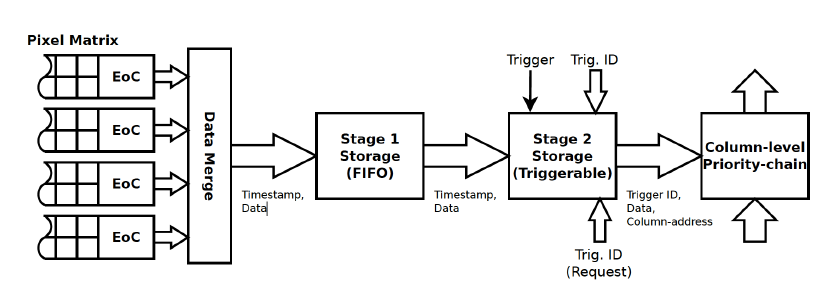
\includegraphics[scale=.8]{obelix_tru}
\caption{Schematic of the Trigger Logic Unit.}
\label{fig:obelix_tru}
\end{figure}

 %In this way, the physics hits associated to a trigger but timestamped with a later BCID, for example due to timewalk effect, are also considered for further analysis.
These components are designed to minimize power dissipation and to optimize the efficiency, even in severe operating conditions: maximum hit rate of \SI{120}{MHz/cm^{2}}, \SI{30}{KHz} of trigger rate and \SI{10}{\micro s} of trigger delay.


\begin{description}
\item \textbf{Track Trigger Transmitter (TTT)}
\end{description}

It is under study the possibility for OBELIX to generate information to be used for a fast track reconstruction at trigger time.
The TTT module divides the matrix in 8 logic regions (this value is still under study) and generates a one-byte word depending on the region firing. It is expected that this information could be transmitted to trigger system within \SI{100}{ns} and along a line of transmission parallel to the main data output of the sensor. 
This component behaviour is still under study and it needs of further simulations in correlation with the whole VTX system.

\newpage
\begin{description}
\item \textbf{Control Unit (CRU) and power dissipation}
\end{description}

%The OBELIX sensor, as well as TJ-Monopix2, is configured by several registers which allow to set important features for its operation like threshold settings, masked pixels, time response of the pixels, but they also define its power consumption.

As well as TJ-Monopix2, the main features of the OBELIX chip operation could be configured by several registers, which allow to determine the threshold settings, masked pixels, time response of the pixels, and which also define its power consumption. The Control Unit is responsible for receiving these configuration instructions and the trigger information, and at the same time, sending out data coming from TXU module.

For what concern power dissipation, there are three main features which have the greatest impact: the biasing current flowing into the in-pixel amplifier (\textit{$I_{BIAS}$}), the BCID clock frequency (on which the timestamping precision depends) and the hit rate. In~\autoref{fig:obelix_power_cons} the estimations of power dissipation varying these parameters is shown.

\begin{figure}[h!]
\centering
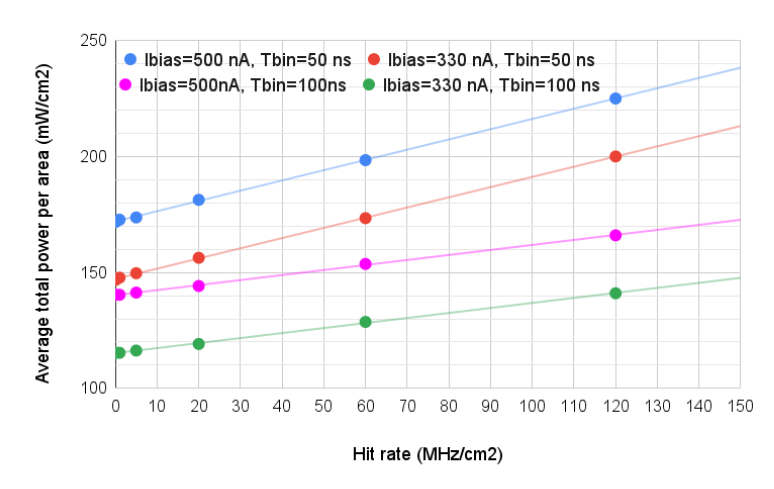
\includegraphics[scale=.8]{obelix_power_cons}
\caption{OBELIX sensor power dissipation depending on the front end current (\textbf{$I_{bias}$}, the BCID frequency (tbin) and the hit rate).}
\label{fig:obelix_power_cons}
\end{figure}

As we can see, the power consumption at the maximum hit rate of \SI{120}{MHz/cm^{2}} exceeds by little more than 10\% the power budget of \SI{200}{mW/cm^{2}}, considering the higher precision for the timestamp of \SI{50}{ns}. Therefore, it is necessary to find a compromise between the value of timing precision and the biasing current to stay within the power budget.
%: reducing timing precision by worsening the BCID precision to 100 ns or decreasing the pre-amplifier biasing current causing a degradation of the time walk.


The first version of the sensor, called OBELIX-1, is being designed. A second improved version, OBELIX-2, will be designed based on performance studies on the first version and it is expected that it will be the final sensor needed for the experiment.
%and the submission for fabrication is planned in the last month of 2023.


\begin{comment}

In this chapter we have introduced some of the fundamental aspects of the proposed VTX upgrade, suppported by continuous studies and simulations. In the following we will see in more details the technology on which the whole proposal is based: the CMOS Monolithic Active Pixel Sensor.

\end{comment}


